% Source: bigram_multinomial_log_reg_gradient_computation.tex
\begin{notechapter}
\chapter{Bigram Logistic Regression: Loss and Gradient}\label{ch:bigram-logreg-gradient}

\section{Introduction}
This document explains the multinomial logistic regression model applied to
bigram language modeling. The goal is to estimate the probability
\( P(\text{word}_2 \mid \text{word}_1) \), where \(\text{word}_1\) is the
previous word and \(\text{word}_2\) is the next word. The model uses a
single-layer neural network with a softmax activation function.

\section{Model Diagram with Bias Term}
The following diagram illustrates the structure of the model, including the
bias term:

\begin{center}
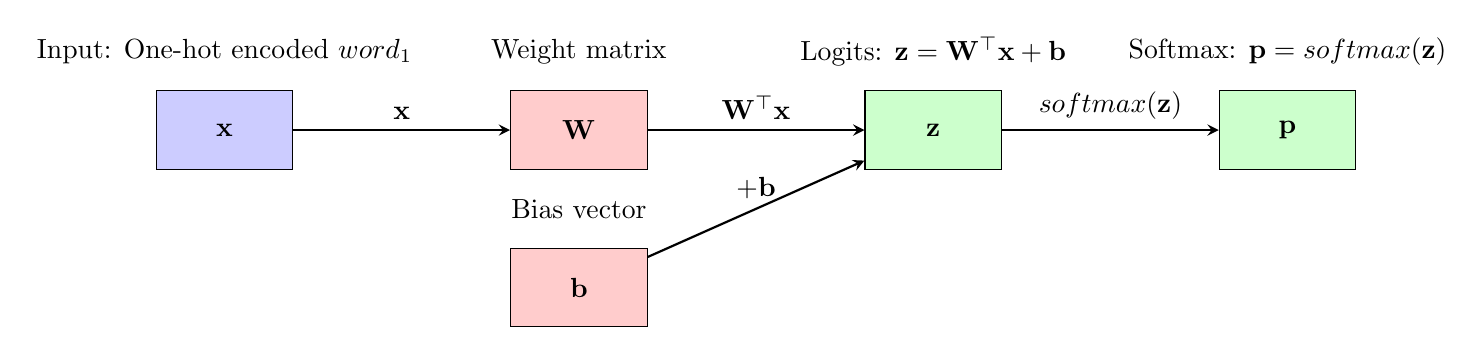
\begin{tikzpicture}[
    node distance=1.5cm,
    input/.style={rectangle, draw, fill=blue!20, text width=1.5cm, 
                  text centered, minimum height=1cm},
    output/.style={rectangle, draw, fill=green!20, text width=1.5cm, 
                   text centered, minimum height=1cm},
    param/.style={rectangle, draw, fill=red!20, text width=1.5cm, 
                  text centered, minimum height=1cm},
    arrow/.style={thick,->,>=stealth}
]
    % Input layer
    \node[input] (x) {$\mathbf{x}$};
    \node[above of=x, yshift=-0.5cm] (input_label) 
          {Input: One-hot encoded $\text{word}_1$};

    % Weight matrix
    \node[param, right of=x, xshift=3cm] (W) {$\mathbf{W}$};
    \node[above of=W, yshift=-0.5cm] (W_label) {Weight matrix};

    % Bias vector
    \node[param, below of=W, yshift=-0.5cm] (b) {$\mathbf{b}$};
    \node[above of=b, yshift=-0.5cm] (b_label) {Bias vector};

    % Logits
    \node[output, right of=W, xshift=3cm] (z) {$\mathbf{z}$};
    \node[above of=z, yshift=-0.5cm] (z_label) 
          {Logits: $\mathbf{z} = \mathbf{W}^\top \mathbf{x} + \mathbf{b}$};

    % Softmax
    \node[output, right of=z, xshift=3cm] (p) {$\mathbf{p}$};
    \node[above of=p, yshift=-0.5cm] (p_label) 
          {Softmax: $\mathbf{p} = \text{softmax}(\mathbf{z})$};

    % Arrows
    \draw[arrow] (x) -- (W) node[midway, above] {$\mathbf{x}$};
    \draw[arrow] (W) -- (z) node[midway, above] {$\mathbf{W}^\top \mathbf{x}$};
    \draw[arrow] (b) -- (z) node[midway, above] {$+ \mathbf{b}$};
    \draw[arrow] (z) -- (p) node[midway, above] {$\text{softmax}(\mathbf{z})$};

\end{tikzpicture}
\end{center}

\subsection{Explanation of the Diagram}
\begin{itemize}
    \item The input \(\mathbf{x}\) is a one-hot encoded vector representing
          \(\text{word}_1\).
    \item The weight matrix \(\mathbf{W}\) maps the input to the logits
          \(\mathbf{z}\).
    \item The bias term \(\mathbf{b}\) adds flexibility to the model by
          allowing it to learn an offset for each output class.
    \item The softmax function converts the logits \(\mathbf{z}\) into
          probabilities \(\mathbf{p}\).
\end{itemize}

\section{Model Diagram without Bias Term}
The following diagram illustrates the structure of the model without the bias
term:


\begin{minipage}[t]{.62\textwidth}
\raggedright
\begin{center}
      \tikzset{%
        every neuron/.style={
          circle,
          draw,
          minimum size=1cm
        },
        neuron missing/.style={
          draw=none, 
          scale=4,
          text height=0.333cm,
          execute at begin node=\color{black}$\vdots$
        },
      }

      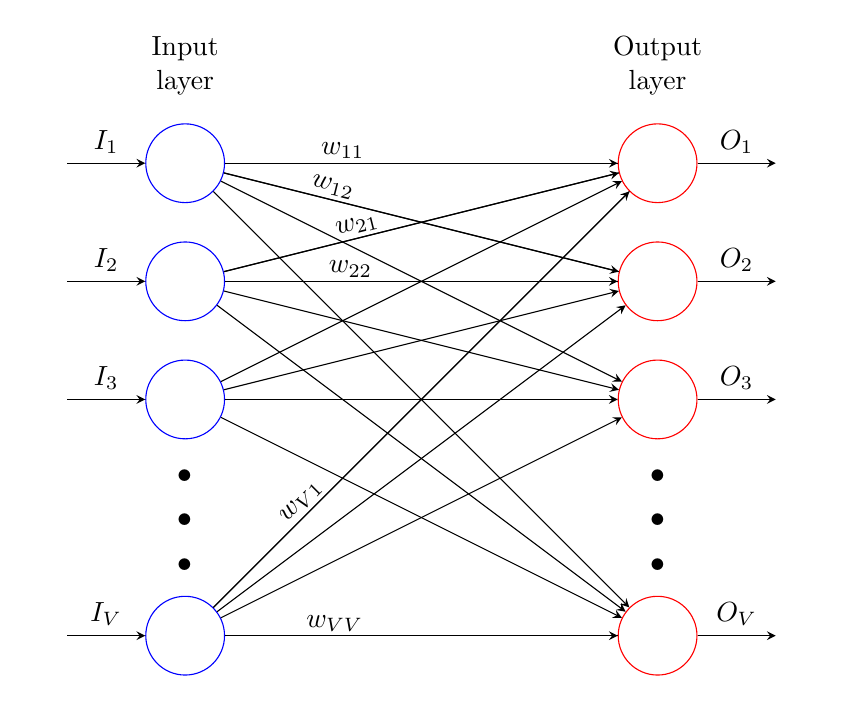
\begin{tikzpicture}[x=1.5cm, y=1.5cm, >=stealth]
      
      \foreach \m/\l [count=\y] in {1,2,3,missing,4}
        \node [every neuron/.try, neuron \m/.try, color=blue] (input-\m) at (0,2.5-\y) {};
      
      \foreach \m [count=\y] in {1,2,3,missing,4}
        \node [every neuron/.try, neuron \m/.try, color=red] (output-\m) at (4,2.5-\y) {};
      
      \foreach \l [count=\i] in {1,2,3,V}
        \draw [<-] (input-\i) -- ++(-1,0)
          node [above, midway] {$I_\l$};
      
      \foreach \l [count=\i] in {1,2,3,V}
        \draw [->] (output-\i) -- ++(1,0)
          node [above, midway] {$O_\l$};
      
      % Label weights only for i=1 and i=V
      \foreach \j in {1,...,4} {
        \draw [->] (input-1) -- (output-\j);
        \draw [->] (input-4) -- (output-\j);
      }
      
      \draw (input-1) -- (output-1)
          node [midway, above, sloped, xshift={-1.0cm}, yshift={-0.07cm}] {$w_{11}$};
      \draw (input-1) -- (output-2)
          node [midway, above, sloped, xshift={-1.2cm}, yshift={-0.07cm}] {$w_{12}$};
          
      \draw (input-2) -- (output-1)
          node [midway, above, sloped, xshift={-0.8cm}, yshift={-0.07cm}] {$w_{21}$};
      
      \draw (input-2) -- (output-2)
          node [midway, above, sloped, xshift={-0.9cm}, yshift={-0.07cm}] {$w_{22}$};
      
      \draw (input-4) -- (output-1)
          node [midway, above, sloped, xshift={-2.0cm}, yshift={-0.07cm}] {$w_{V1}$};
      \draw (input-4) -- (output-4)
          node [midway, above, sloped, xshift={-1.1cm}, yshift={-0.07cm}] {$w_{VV}$};
      
      % Draw connections for i=2 and i=3 without labels
      \foreach \i in {2,3}
        \foreach \j in {1,...,4}
          \draw [->] (input-\i) -- (output-\j);
      
      \foreach \l [count=\x from 0] in {Input, Output}
        \node [align=center, above] at (\x*4,2) {\l \\ layer};
      
      \end{tikzpicture}
      \end{center}
\end{minipage}
\hfill
\noindent
\begin{minipage}[t]{.34\textwidth}
\raggedleft
\[
\mathbf{x} = 
\begin{bmatrix}
x_1 = I_{1} \\
x_2 = I_{2} \\
\vdots \\
x_V = I_{V}
\end{bmatrix}
\]

\[
\mathbf{W} = 
\begin{bmatrix}
w_{11} & w_{12} & \cdots & w_{1V} \\
w_{21} & w_{22} & \cdots & w_{2V} \\
\vdots & \vdots & \ddots & \vdots \\
w_{V1} & w_{V2} & \cdots & w_{VV}
\end{bmatrix}
\] 

\[
\mathbf{W}^\top \mathbf{x} = 
\begin{bmatrix}
w_{11} I_1 + w_{21} I_2 + \cdots + w_{V1} I_V \\
w_{12} I_1 + w_{22} I_2 + \cdots + w_{V2} I_V \\
\vdots \\
w_{1V} I_1 + w_{2V} I_2 + \cdots + w_{VV} I_V
\end{bmatrix}
\]
\end{minipage}

\subsection{Explanation of the Diagram}
\begin{itemize}
    \item The input layer consists of \( V \) neurons, where \( V \) is the
          vocabulary size. Each neuron corresponds to a one-hot encoded input
          \( I_1, I_2, \dots, I_V \). For example, if \(\text{word}_1\) is the
          \(i\)-th word in the vocabulary, then \( I_i = 1 \) and all other
          \( I_j = 0 \).\\
          Therefore, $\mathbf{W}^\top \mathbf{x}$ is equal to the transpose
          of the $i^{\text{th}}$ line of the matrix $\mathbf{W}$.\\
          For example,
          \[
            \mathbf{W}^{T} \mathbf{x} = 
            \begin{bmatrix}
            w_{11} & w_{21} & \cdots & w_{V1} \\
            w_{12} & w_{22} & \cdots & w_{V2} \\
            \vdots & \vdots & \ddots & \vdots \\
            w_{1V} & w_{2V} & \cdots & w_{VV}
            \end{bmatrix}
            \begin{bmatrix}
                  1 \\
                  0 \\
                  \vdots \\
                  0
            \end{bmatrix} =
            \begin{bmatrix}
                  w_{11} \\ w_{12} \\ \vdots \\ w_{1V}
            \end{bmatrix}
            \]
    \item The output layer also consists of \( V \) neurons, representing the
          output probabilities \( O_1, O_2, \dots, O_V \). These probabilities
          are computed using the softmax function:
          \[
          O_j = P(\text{word}_2 = j \mid \text{word}_1) =
          \text{softmax}(\mathbf{z})_j = \frac{e^{z_j}}{\sum_{k=1}^V e^{z_k}}.
          \]
    \item The connections between the input and output layers represent the
          weight matrix \(\mathbf{W}\), which maps the input to the logits
          \(\mathbf{z}\).
\end{itemize}

\section{Loss Function}
The model is trained using the \textbf{cross-entropy loss}. For a single
training example \((\text{word}_1, \text{word}_2)\), the loss is defined as:
\[
\mathcal{L} = -\log P(\text{word}_2 \mid \text{word}_1).
\]
This formula is a special case of the cross-entropy loss, which measures
the difference between the true distribution and the predicted distribution.

\subsection{True Distribution}
In reality, the true distribution of \(\text{word}_2\) given \(\text{word}_1\)
is not a one-hot vector. Instead, it is a probability distribution over the
vocabulary, where each word \(j\) has a probability \(y_j\) of being the next
word given \(\text{word}_1\). For example, if \(\text{word}_1\) is "the", then
\(\text{word}_2\) could be "cat", "dog", "house", etc., each with a certain
probability.

However, in practice, we often approximate the true distribution using a
\textbf{one-hot encoded vector} for computational simplicity. In this
approximation:
\begin{itemize}
    \item The true word \(\text{word}_2\) is assigned a probability of 1.
    \item All other words are assigned a probability of 0.
\end{itemize}

This simplification is justified because, during training, we typically treat
each \((\text{word}_1, \text{word}_2)\) pair as an independent observation.
The model is trained to maximize the likelihood of the observed \(\text{word}_2\)
given \(\text{word}_1\), even though multiple valid \(\text{word}_2\) values
may exist for a given \(\text{word}_1\) in the corpus.

\subsection{Predicted Distribution}
The predicted distribution is the model's output probability vector
\(\mathbf{p}\), computed using the softmax function:
\[
p_j = P(\text{word}_2 = j \mid \text{word}_1) =
\text{softmax}(\mathbf{z})_j = \frac{e^{z_j}}{\sum_{k=1}^V e^{z_k}}.
\]
Here, \(\mathbf{z}\) is the logit vector computed as:
\[
\mathbf{z} = \mathbf{W}^\top \mathbf{x} + \mathbf{b},
\]
where \(\mathbf{x}\) is the one-hot encoded input vector for \(\text{word}_1\).

\subsection{Cross-Entropy Loss}
The cross-entropy loss measures the difference between the true distribution
\(\mathbf{y}\) (one-hot encoded) and the predicted distribution \(\mathbf{p}\):
\[
\mathcal{L} = -\sum_{j=1}^V y_j \log p_j.
\]
Since \(\mathbf{y}\) is one-hot encoded (with \(y_j = 1\) for the true word
and \(y_j = 0\) for all other words), the loss simplifies to:
\[
\mathcal{L} = -\log p_{\text{target\_idx}},
\]
where \(p_{\text{target\_idx}}\) is the predicted probability for the true
word \(\text{word}_2\).

\subsection{Justification of the Simplification}
While the true distribution of \(\text{word}_2\) given \(\text{word}_1\) is
not a one-hot vector, the one-hot approximation is commonly used in practice
because:
\begin{itemize}
    \item \textbf{Computational Efficiency}: Working with one-hot vectors
          simplifies the computation of the loss and its gradients.
    \item \textbf{Maximum Likelihood Estimation}: The model is trained to
          maximize the likelihood of the observed \(\text{word}_2\) given
          \(\text{word}_1\), which aligns with the one-hot approximation.
    \item \textbf{Empirical Success}: Despite the simplification, this
          approach has been empirically successful in many natural language
          processing tasks.
\end{itemize}

However, it is important to note that this simplification ignores the fact
that multiple words can follow \(\text{word}_1\) in valid bigrams. In more
advanced models, such as those using \textbf{label smoothing} or
\textbf{distributional targets}, the true distribution is modeled more
accurately.

\section{Gradient Computation}
The gradients of the loss with respect to the parameters \(\mathbf{W}\) and
\(\mathbf{b}\) are computed using backpropagation.

\subsection{Gradient of the Loss with Respect to the Logits}
The logits \(\mathbf{z}\) are the outputs of the linear transformation:
\[
\mathbf{z} = \mathbf{W}^\top \mathbf{x} + \mathbf{b}.
\]
The gradient of the cross-entropy loss with respect to the logits is:
\[
\frac{\partial \mathcal{L}}{\partial z_j} = p_j - \mathbb{I}(j = \text{target\_idx}),
\]
where:
\begin{itemize}
    \item \( p_j \) is the predicted probability for the \( j \)-th word.
    \item \( \mathbb{I}(j = \text{target\_idx}) \) is an indicator function
          that is 1 if \( j = \text{target\_idx} \) and 0 otherwise.
\end{itemize}

\subsection{Derivation of \(\frac{\partial \mathcal{L}}{\partial z_j}\)}
The cross-entropy loss for a single training example is:
\[
\mathcal{L} = -\log p_{\text{target\_idx}},
\]
where \( p_{\text{target\_idx}} \) is the predicted probability for the true
target word. The softmax function is defined as:
\[
p_j = \frac{e^{z_j}}{\sum_{k=1}^V e^{z_k}}.
\]
To compute \(\frac{\partial \mathcal{L}}{\partial z_j}\), we use the chain rule:
\[
\frac{\partial \mathcal{L}}{\partial z_j} = 
\frac{\partial \mathcal{L}}{\partial p_{\text{target\_idx}}} 
\cdot \frac{\partial p_{\text{target\_idx}}}{\partial z_j}.
\]
First, compute \(\frac{\partial \mathcal{L}}{\partial p_{\text{target\_idx}}}\):
\[
\frac{\partial \mathcal{L}}{\partial p_{\text{target\_idx}}} = 
-\frac{1}{p_{\text{target\_idx}}}.
\]
Next, compute \(\frac{\partial p_{\text{target\_idx}}}{\partial z_j}\):
\[
\frac{\partial p_{\text{target\_idx}}}{\partial z_j} = 
p_{\text{target\_idx}} (\mathbb{I}(j = \text{target\_idx}) - p_j).
\]
Combining these results:
\[
\frac{\partial \mathcal{L}}{\partial z_j} = 
-\frac{1}{p_{\text{target\_idx}}} \cdot 
p_{\text{target\_idx}} (\mathbb{I}(j = \text{target\_idx}) - p_j) 
= p_j - \mathbb{I}(j = \text{target\_idx}).
\]

\subsection{Gradient of the Loss with Respect to \(\mathbf{W}\)}
The weight matrix \(\mathbf{W}\) is used to compute the logits
\(\mathbf{z} = \mathbf{W}^\top \mathbf{x} + \mathbf{b}\). To compute the
gradient of the loss \(\mathcal{L}\) with respect to \(\mathbf{W}\), we use
the chain rule. Here is the detailed derivation:

\subsubsection{Step 1: Express the Loss in Terms of \(\mathbf{W}\)}
The loss \(\mathcal{L}\) is a function of the predicted probabilities \(\mathbf{p}\),
which in turn depend on the logits \(\mathbf{z}\). The logits \(\mathbf{z}\) are
computed as:
\[
\mathbf{z} = \mathbf{W}^\top \mathbf{x} + \mathbf{b}.
\]
Thus, the loss \(\mathcal{L}\) depends on \(\mathbf{W}\) through \(\mathbf{z}\).

\subsubsection{Step 2: Apply the Chain Rule}
Using the chain rule, the gradient of the loss with respect to \(\mathbf{W}\) is:
\[
\frac{\partial \mathcal{L}}{\partial \mathbf{W}} = 
\frac{\partial \mathcal{L}}{\partial \mathbf{z}} \cdot 
\frac{\partial \mathbf{z}}{\partial \mathbf{W}}.
\]

\subsubsection{Step 3: Compute \(\frac{\partial \mathcal{L}}{\partial \mathbf{z}}\)}
From the previous section, we have:
\[
\frac{\partial \mathcal{L}}{\partial z_j} = p_j - \mathbb{I}(j = \text{target\_idx}),
\]
where:
\begin{itemize}
\item \( p_j \) is the predicted probability for the \( j \)-th word;
\item \( \mathbb{I}(j = \text{target\_idx}) \) is an indicator function that is 1 if
  \( j = \text{target\_idx} \) and 0 otherwise.
\end{itemize}

Thus, the gradient of the loss with respect to \(\mathbf{z}\) is:
\[
\frac{\partial \mathcal{L}}{\partial \mathbf{z}} = 
\begin{bmatrix}
p_1 - \mathbb{I}(1 = \text{target\_idx}) \\
p_2 - \mathbb{I}(2 = \text{target\_idx}) \\
\vdots \\
p_V - \mathbb{I}(V = \text{target\_idx})
\end{bmatrix}.
\]

\subsubsection{Step 4: Compute \(\frac{\partial \mathbf{z}}{\partial \mathbf{W}}\)}
The logits \(\mathbf{z}\) are computed as:
\[
\mathbf{z} = \mathbf{W}^\top \mathbf{x} + \mathbf{b}.
\]
To compute \(\frac{\partial \mathbf{z}}{\partial \mathbf{W}}\),
we differentiate \(\mathbf{z}\) with respect to each element of
\(\mathbf{W}\). Let \(\mathbf{W} \in \mathbb{R}^{d \times V}\),
where \(d\) is the input dimension and \(V\) is the vocabulary size.
Then:
\[
\frac{\partial z_j}{\partial W_{ij}} = x_i \cdot \mathbb{I}(k = j),
\]
where \(\mathbb{I}(k = j)\) is an indicator function that is 1 if
\(k = j\) and 0 otherwise.

Thus, the gradient \(\frac{\partial \mathbf{z}}{\partial \mathbf{W}}\)
is a \textbf{3D tensor} of size \(V \times d \times V\), where:
\[
\frac{\partial z_j}{\partial W_{ik}} = x_i \cdot \mathbb{I}(k = j).
\]

\subsubsection{Step 5: Combine the Results}
Using the chain rule, the gradient of the loss with respect to
\(\mathbf{W}\) is:
\[
\frac{\partial \mathcal{L}}{\partial W_{ij}} = 
\sum_{k=1}^V \frac{\partial \mathcal{L}}{\partial z_k} \cdot \frac{\partial z_k}{\partial W_{ij}}.
\]
Substituting \(\frac{\partial z_k}{\partial W_{ij}} = x_i \cdot \mathbb{I}(k = j)\), we have:
\[
\frac{\partial \mathcal{L}}{\partial W_{ij}} = 
\frac{\partial \mathcal{L}}{\partial z_j} \cdot x_i.
\]

Thus, the gradient of the loss with respect to \(\mathbf{W}\) is:
\begin{align*}
    \frac{\partial \mathcal{L}}{\partial \mathbf{W}} =
    \begin{bmatrix}
        \frac{\partial \mathcal{L}}{\partial W_{11}} &
        \frac{\partial \mathcal{L}}{\partial W_{12}} & 
        \cdots &
        \frac{\partial \mathcal{L}}{\partial W_{1V}} \\[6pt]
        \frac{\partial \mathcal{L}}{\partial W_{21}} &
        \frac{\partial \mathcal{L}}{\partial W_{22}} & 
        \cdots &
        \frac{\partial \mathcal{L}}{\partial W_{2V}} \\
        \vdots & \vdots & \ddots & \vdots \\
        \frac{\partial \mathcal{L}}{\partial W_{V1}} &
        \frac{\partial \mathcal{L}}{\partial W_{V2}} & 
        \cdots &
        \frac{\partial \mathcal{L}}{\partial W_{VV}} 
    \end{bmatrix} 
    =
    \begin{bmatrix}
        \frac{\partial \mathcal{L}}{\partial z_{1}} x_1 &
        \frac{\partial \mathcal{L}}{\partial z_{2}} x_1 & 
        \cdots &
        \frac{\partial \mathcal{L}}{\partial z_{V}} x_1\\[6pt]
        \frac{\partial \mathcal{L}}{\partial z_{1}} x_2 &
        \frac{\partial \mathcal{L}}{\partial z_{2}} x_2 & 
        \cdots &
        \frac{\partial \mathcal{L}}{\partial z_{V}} x_2\\
        \vdots & \vdots & \ddots & \vdots \\
        \frac{\partial \mathcal{L}}{\partial z_{1}} x_V &
        \frac{\partial \mathcal{L}}{\partial z_{2}} x_V & 
        \cdots &
        \frac{\partial \mathcal{L}}{\partial z_{V}} x_V
    \end{bmatrix}
    =
    \begin{bmatrix}
        x_1\\[6pt]
        x_2\\
        \vdots \\
        x_V
    \end{bmatrix}
    \begin{bmatrix}
        \frac{\partial \mathcal{L}}{\partial z_{1}} &
        \frac{\partial \mathcal{L}}{\partial z_{2}} & 
        \cdots &
        \frac{\partial \mathcal{L}}{\partial z_{V}} 
    \end{bmatrix}
\end{align*}

That is,
\[
    \frac{\partial \mathcal{L}}{\partial \mathbf{W}}
=
\mathbf{x} \cdot \left( \frac{\partial \mathcal{L}}
{\partial \mathbf{z}} \right)^\top.
\]

\subsection{Gradient of the Loss with Respect to \(\mathbf{b}\)}
The bias vector \(\mathbf{b}\) is added to the logits
\(\mathbf{z} = \mathbf{W}^\top \mathbf{x} + \mathbf{b}\). The gradient of the
loss with respect to \(\mathbf{b}\) is simply:
\[
\frac{\partial \mathcal{L}}{\partial \mathbf{b}} = 
\frac{\partial \mathcal{L}}{\partial \mathbf{z}}.
\]

\section{Example}
Suppose:
\begin{itemize}
    \item Vocabulary size \( V = 3 \).
    \item Input vector \(\mathbf{x} = [1, 0, 0]^\top\) (one-hot encoded for
          the first word).
    \item Predicted probabilities \(\mathbf{p} = [0.1, 0.7, 0.2]^\top\).
    \item Target index \(\text{target\_idx} = 1\) (the correct next word is
          the second word).
\end{itemize}

\subsection{Compute \(\frac{\partial \mathcal{L}}{\partial \mathbf{z}}\)}
\[
\frac{\partial \mathcal{L}}{\partial \mathbf{z}} = 
[0.1, 0.7, 0.2]^\top - [0, 1, 0]^\top = [0.1, -0.3, 0.2]^\top.
\]

\subsection{Compute \(\frac{\partial \mathcal{L}}{\partial \mathbf{W}}\)}
\[
\frac{\partial \mathcal{L}}{\partial \mathbf{W}} = 
\mathbf{x} \cdot \left( \frac{\partial \mathcal{L}}{\partial \mathbf{z}} \right)^\top = 
\begin{bmatrix}
1 \\ 0 \\ 0
\end{bmatrix}
\cdot
\begin{bmatrix}
0.1 & -0.3 & 0.2
\end{bmatrix}
=
\begin{bmatrix}
0.1 & -0.3 & 0.2 \\
0 & 0 & 0 \\
0 & 0 & 0
\end{bmatrix}.
\]

\subsection{Compute \(\frac{\partial \mathcal{L}}{\partial \mathbf{b}}\)}
\[
\frac{\partial \mathcal{L}}{\partial \mathbf{b}} = 
[0.1, -0.3, 0.2]^\top.
\]

\section{Python Implementation}
Below is the Python implementation of the gradient computation using NumPy.

\begin{verbatim}
import numpy as np

def compute_gradients(x, p, target_idx):
    # Compute the gradient of the loss with respect to the logits
    dL_dz = p.copy()
    dL_dz[target_idx] -= 1  # Subtract 1 at the target index

    # Compute the gradient of the loss with respect to W
    dL_dW = np.outer(x, dL_dz)

    # Compute the gradient of the loss with respect to b
    dL_db = dL_dz

    return dL_dW, dL_db
\end{verbatim}

\section{Conclusion}
The gradient computation for multinomial logistic regression in bigram language
modeling involves calculating the gradients of the loss with respect to the
logits, weight matrix \(\mathbf{W}\), and bias vector \(\mathbf{b}\). The
outer product \(\mathbf{x} \cdot \left( \frac{\partial \mathcal{L}}{\partial \mathbf{z}} \right)^\top\)
is used to compute the gradient of the loss with respect to \(\mathbf{W}\),
ensuring that the dimensions align correctly.
\end{notechapter}
